\documentclass[a4paper,10pt]{article} 
\usepackage[utf8]{inputenc}
\usepackage[a4paper]{geometry}
\usepackage[magyar]{babel}
\usepackage{amsmath}
\usepackage{amssymb}
\usepackage{pgf,tikz}
\frenchspacing 
\pagestyle{empty}
\newcommand{\ki}[2]{\hfill {\it #1 (#2)}\medskip}
\newcommand{\vonal}{\hbox to \hsize{\hskip2truecm\hrulefill\hskip2truecm}}
\newcommand{\degre}{\ensuremath{^\circ}}
\newcommand{\tg}{\mathop{\mathrm{tg}}\nolimits}
\newcommand{\ctg}{\mathop{\mathrm{ctg}}\nolimits}
\newcommand{\arc}{\mathop{\mathrm{arc}}\nolimits}
\begin{document}
\begin{center} \Large {\em 24. Nemzetközi Magyar Matematika Verseny} \end{center}
\begin{center} \large{\em Szabadka, 2015. április 8-12.} \end{center}
\smallskip
\begin{center} \large{\bf 12. osztály} \end{center}
\bigskip 

{\bf 1. feladat: } A szabályos hatoldalú csonka gúla alapélei $a$ és $b$ ( $a > b$ ). A csonka gúla
oldalfelülete megegyezik az alaplapok területének összegével. Határozd meg a csonka gúla magasságát!

\ki{Angyal Andor}{Szabadka, Vajdaság}\medskip

{\bf Megoldás: } Mivel a csonkagúla oldalfelülete megegyezik az alaplapok területének összegével, ezért
$$6\cdot\frac{(a+b)h}{2}=6\cdot\frac{a^2\sqrt 3}{4}+6\cdot\frac{b^2\sqrt 3}{4}$$
ahol $h$ a csonkagúla oldalmagassága. Rendezés után azt kapjuk, hogy
$$h=\frac{\sqrt 3}{2}\cdot\frac{a^2+b^2}{a+b}.$$
Ha $H$-val jelöljük a csonkagúla testmagasságát, akkor a Pitagorasz-tétel alkalmazásával a
$$h^2=H^2+\left(\frac{a\sqrt 3}{2}-\frac{b\sqrt 3}{2}\right)^2$$
egyenlőséghez jutunk, ahonnan a következő módon kapjuk meg a keresett magasságot:
$$H^2=h^2-\left(\frac{a\sqrt 3}{2}-\frac{b\sqrt 3}{2}\right)^2=
\frac{3}{4}\frac{(a^2+b^2)^2}{(a+b)^2}-\frac{3}{4}(a-b)^2=
\frac{3}{4}\cdot\frac{4a^2b^2}{(a+b)^2}.$$
Gyökvonás után adódik, hogy $H=\dfrac{ab\sqrt 3}{a+b}$.

\vonal

{\bf 2. feladat: } Egy $9 \times 9$-es négyzetrácsba beírtuk a számokat 1-től 81-ig. Bizonyítsd be,
hogy a számok bármely elrendeződése mellett van két olyan szomszédos négyzet,
amelyben a számok közötti különbség legalább 6. (Szomszédosnak tekintjük
azokat a négyzeteket, amelyeknek közös oldaluk van.)

\ki{Béres Zoltán}{Szabadka, Vajdaság}\medskip

{\bf Megoldás: } Tekintsük azt a két négyzetet, amelybe az 1-es és a 81-es van beírva, és keressük a legrövidebb utat a szomszédos négyzeteken keresztül a két szám között. Figyeljük meg, hogy ezen az úton, hány ,,lépéssel'' tudunk végigmenni.  

\textit{1. eset}. Az 1-es és a 81-es a két átellenes sarokban van. Ekkor a legrövidebb út a két négyzet között 16 lépésből áll (8 jobbra és 8 balra), és létezik két ilyen út is, amelyeknek nincs közös négyzetük.

Ha feltesszük, hogy nincs 5-nél nagyobb különbség a szomszédos mezők között, akkor az út négyzeteibe írt egyetlen lehetséges számsor az 1, 6, 11, 16, 21,\ldots, 71, 76, 81, ahol a szomszédos számok közötti különbség mindig 5. Ekkor a másik út, mely ezeket a számokat nem tartalmazhatja, szükségképpen tartalmaz egy 5-ösnél nagyobb lépést, mivel a második szám csak 6-nál kisebb lehet, és a további lehető legnagyobb, 5-ös lépésekkel sem érheti el a 81-et.

\textit{2. eset}.  Az 1-es és a 81-es nem a két átellenes sarokban van. Ekkor a legrövidebb út a két négyzet között rövidebb, mint 16 lépés. Ha feltesszük, hogy nincs 5-nél nagyobb különbség a szomszédos mezők között, akkor legfeljebb 15 lépésből az elérhető legnagyobb szám a 76, így nem érhetjük el a 81-et.

\vonal


{\bf 3. feladat: } Ha $\alpha$ hegyesszög, akkor bizonyítsd be, hogy teljesül az
$$\left(1+\frac{1}{\sin \alpha}\right)\cdot\left(1+\frac{1}{\cos \alpha}\right)\ge 3+2\sqrt 2$$
egyenlőtlenség!

\ki{Csikós Pajor Gizella}{Szabadka, Vajdaság}\medskip

{\bf Megoldás: } Végezzük el a következő átalakításokat, alkalmazva a számtani és mértani közepek közötti összefüggést, valamint azt, hogy 
$|\sin x|\le 1$:

\begin{align*}
~&\left(1+\frac{1}{\sin \alpha}\right)\cdot
\left(1+\frac{1}{\cos \alpha}\right)=
1+\left(\frac{1}{\sin \alpha}+\frac{1}{\sin \alpha}\right)+\frac{1}{\sin \alpha \cos \alpha}\ge\\
&\ge 1+\frac{2}{\sqrt{\sin \alpha \cos \alpha}}+
\frac{1}{\sin \alpha \cos \alpha} =
\left(1+\frac{1}{\sqrt{\sin \alpha \cos \alpha}}\right)^2 =
\left(1+\frac{\sqrt 2}{\sqrt{2\sin \alpha \cos \alpha}}\right)^2=\\
&=\left(1+\frac{\sqrt 2}{\sqrt{\sin 2\alpha}}\right)^2\ge (1+\sqrt 2)^2=1+2\sqrt 2+2 =
3+2\sqrt 2.
\end{align*}

\vonal


{\bf 4. feladat: } Oldd meg a következő egyenletet a valós számok halmazán:
$$(2x+1)\sqrt{(2x-1)^3}+16x^4=2x(4x-1).$$

\ki{Olosz Ferenc}{Szatmárnémeti, Erdély}\medskip

{\bf 1. megoldás: } Az egyenlet értelmezett, ha 
$x\in\left[\frac{1}{2};\infty\right)$.
Az egyenletet balra rendezzük, majd 1 hozzáadásával és kivonásával a
$$(2x-1)+(2x+1)(2x-1)\sqrt{2x-1}+(16x^4-8x^2+1)=0,$$
illetve
$$\left(\sqrt{2x-1}\right)^2+(4x^2-1)\sqrt{2x-1}+
(4x^2-1)^2=0$$
alakra hozzuk. 
A valós számok halmazán az $a^2\pm ab+b^2=0$  akkor és csak akkor teljesül, ha $a=b=0$. Esetünkben keressük a $\sqrt{2x-1}=0$ és $4x^2-1=0$ egyenletek közös megoldását és ez $x=\dfrac{1}{2}$.

{\bf 2. megoldás: } Az egyenlet értelmezett, ha 
$2x-1\ge 0$, vagyis $x\in\left[\frac{1}{2};\infty\right)$.  Alkalmazzuk az egyenletre a következő ekvivalens átalakításokat:

\begin{align*}
(2x-1)+(2x+1)(2x-1)\sqrt{2x-1}+(16x^4-8x^2+1)&=0\\
(2x-1)+(2x+1)(2x-1)\sqrt{2x-1}+(4x^2-1)^2&=0\\
(2x-1)+(2x+1)(2x-1)\sqrt{2x-1}+(2x-1)^2(2x+1)^2&=0\\
(2x-1)\left[
1+(2x+1)\sqrt{2x-1}+(2x-1)(2x+1)^2
\right]&=0.
\end{align*}

Minden $x\ge \frac{1}{2}$ esetén 
$1+(2x+1)\sqrt{2x-1}+(2x-1)(2x+1)^2\ge 1$, tehát csak $2x-1$ lehetséges, azaz $x=\dfrac{1}{2}$.

\vonal


{\bf 5. feladat: } Oldd meg a következő egyenletet a valós számok halmazán:
$$2x^2+\sqrt{2}+\log_2^2\left(2x^2+\sqrt 2\right)=2^{\frac{\sqrt{x^2+1}}{x^2+2}}+\frac{x^2+1}{(x^2+2)^2}$$
\ki{Bence Mihály}{Brassó, Erdély}\medskip

{\bf Megoldás: } Mivel nemnegatív értékekre az  $f(x)=2^x+x^2$ függvény szigorúan monoton növekvő, ezért nemnegatív értékekre injektív is. Felhasználva ezt a jelölést az adott egyenlet ekvivalens az 
$$
f\left(\log_2\left(2x^2+\sqrt{2}\right)\right)=
f\left(\frac{\sqrt{x^2+1}}{x^2+2}\right)
$$
egyenlettel, ahonnan az $f$ függvény injektív tulajdonsága miatt következik, hogy
$$\log_2\left(2x^2+\sqrt{2}\right)=\frac{\sqrt{x^2+1}}{x^2+2}.$$
Mivel $\left(\sqrt{x^2+1}-1\right)^2\ge 0$, ahonnan következik 
$$x^2+1-2\sqrt{x^2+1}+1\ge 0,$$
valamint 
$$x^2+2-2\sqrt{x^2+1}\ge 0,$$
illetve a 
$$2\sqrt{x^2+1}\le x^2+2$$
egyenlőtlenség, így érvényes, hogy
$$
\frac{\sqrt{x^2+1}}{x^2+2}\le \frac{1}{2} 
\text{~és~} 
\log_2\left(2x^2+\sqrt 2\right)\ge \log_2 \sqrt{2} =\frac{1}{2}
. 
$$
Ebből adódik, hogy csak a 
$\dfrac{\sqrt{x^2+1}}{x^2+2}=\dfrac{1}{2}$ egyenlőség lehetséges. 
Ekvivalens átalakításokkal megkapjuk, hogy 
$$2\sqrt{x^2+1}=x^2+2,$$
ahonnan négyzetre emelve mindkét oldalt a 
$$4(x^2+1)=(x^2+2)^2$$
egyenlet következik. Elvégezve a műveleteket, majd rendezve a kapott kifejezést adódik, hogy
$$4x^2+4=x^4+4x^2+4,$$
illetve $x^4=0$, amely egyenlet egyetlen megoldása $x=0$.

\vonal


{\bf 6. feladat: } Egy $\overline{AB}=42$~cm és egy $\overline{CD}=58$~cm hosszú szakasz $\alpha$ szög alatt metszi
egymást az $O$ pontban. Mekkora a szakaszok végpontjaival (mint csúcsokkal)
alkotott $ACBD$ négyszög pontos területe, ha tudjuk, hogy 
$\tg\dfrac{\alpha}{2}=\dfrac{3}{7}$?

\ki{Gecse Frigyes}{Kisvárda, Magyarország}\medskip


{\bf Megoldás: } Legyenek $E, F, G, H$ az $ABCD$ négyszög oldalainak felezőpontjai. 
A megszámozott alakzatok területét jelöljük $t$-vel, megfelelő indexszel ellátva. 

\begin{center}
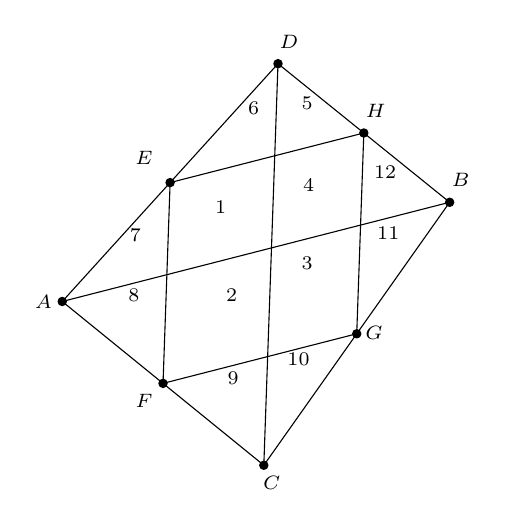
\begin{tikzpicture}[line cap=round,line join=round,x=1.0cm,y=1.0cm]
%\clip(-3.24,-0.02) rectangle (3.18,6.12);
\draw (-2.66,2.62)-- (0.08,5.64);
\draw (0.08,5.64)-- (2.26,3.88);
\draw (2.26,3.88)-- (-0.1,0.54);
\draw (-0.1,0.54)-- (-2.66,2.62);
\draw (-2.66,2.62)-- (2.26,3.88);
\draw (0.08,5.64)-- (-0.1,0.54);
\draw (-1.29,4.13)-- (1.17,4.76);
\draw (1.17,4.76)-- (1.08,2.21);
\draw (1.08,2.21)-- (-1.38,1.58);
\draw (-1.38,1.58)-- (-1.29,4.13);
\begin{scriptsize}
\draw (-0.82,4.) node[anchor=north west] {$1$};
\draw (-0.68,2.88) node[anchor=north west] {$2$};
\draw (0.28,3.28) node[anchor=north west] {$3$};
\draw (0.3,4.28) node[anchor=north west] {$4$};
\draw (0.28,5.32) node[anchor=north west] {$5$};
\draw (-0.4,5.26) node[anchor=north west] {$6$};
\draw (-1.9,3.64) node[anchor=north west] {$7$};
\draw (-1.92,2.88) node[anchor=north west] {$8$};
\draw (-0.66,1.82) node[anchor=north west] {$9$};
\draw (0.1,2.06) node[anchor=north west] {$10$};
\draw (1.24,3.66) node[anchor=north west] {$11$};
\draw (1.2,4.44) node[anchor=north west] {$12$};
\draw [fill=black] (-2.66,2.62) circle (1.5pt);
\draw[color=black] (-2.9,2.62) node {$A$};
\draw [fill=black] (2.26,3.88) circle (1.5pt);
\draw[color=black] (2.4,4.16) node {$B$};
\draw [fill=black] (-0.1,0.54) circle (1.5pt);
\draw[color=black] (0.,0.32) node {$C$};
\draw [fill=black] (0.08,5.64) circle (1.5pt);
\draw[color=black] (0.22,5.92) node {$D$};
\draw [fill=black] (-1.29,4.13) circle (1.5pt);
\draw[color=black] (-1.62,4.44) node {$E$};
\draw [fill=black] (1.17,4.76) circle (1.5pt);
\draw[color=black] (1.32,5.04) node {$H$};
\draw [fill=black] (1.08,2.21) circle (1.5pt);
\draw[color=black] (1.3,2.22) node {$G$};
\draw [fill=black] (-1.38,1.58) circle (1.5pt);
\draw[color=black] (-1.62,1.36) node {$F$};
\end{scriptsize}
\end{tikzpicture}
\end{center}

A keresett $t_{ABCD}$ területre fennáll a 
$t_{ABCD}=t_1+t_2+\ldots+t_{11}+t_{12}$ egyenlőség. Az $EFGH$ négyszög paralelogramma, mert egy-egy oldalpárja párhuzamos egy megfelelő adott szakasszal. Mint háromszögek középvonalai
$$
\overline{EH}=\frac{1}{2}\overline{AB}=21\text{~cm},
\overline{HG}=\frac{1}{2}\overline{CD}=29\text{~cm} .$$
Tudjuk (ha nem a paralelogrammára, akkor a háromszögre vonatkozóan), hogy
$$t_{EFGH}=\overline{EH}\cdot\overline{HG}\cdot \sin \alpha=21\cdot 29\cdot \sin \alpha.$$
A háromszögek középvonalainak és a paralelogramma átlóinak tulajdonságait felhasználva adódik, 
hogy 
$t_1=t_6+t_7$, 
$t_2=t_8+t_9$, 
$t_3=t_{10}+t_{11}$,
$t_4=t_5+t_{12}$. Innen
$$t_{EFGH}=t_1+t_2+t_3+t_4=t_5+t_6+\ldots+t_{12}
=21\cdot 29\cdot \sin \alpha.$$
Ennélfogva
$$t_{ABCD}=2(t_1+t_2+t_3+t_4)=2\cdot 21\cdot 29\cdot \sin \alpha.$$
Az ismert 
$$\sin \alpha = \frac{2\tg \frac{\alpha}{2}}{1+\tg^2\frac{\alpha}{2}}$$
képlet alapján (ha nem ismerjük, vezessük le) adódik, hogy 
$$\sin \alpha = \frac{2\cdot \frac{3}{7}}{1+\frac{9}{49}}=\frac{21}{29}.$$
Végül $t_{ABCD}=2\cdot 21\cdot 29\cdot \frac{21}{29}=2\cdot 21^2=882\text{~cm}^2$.


\end{document}